\subsubsection{Activity Diagram - Chức năng tạo đợt đóng phí}

\begin{figure}[H]
        \centering
        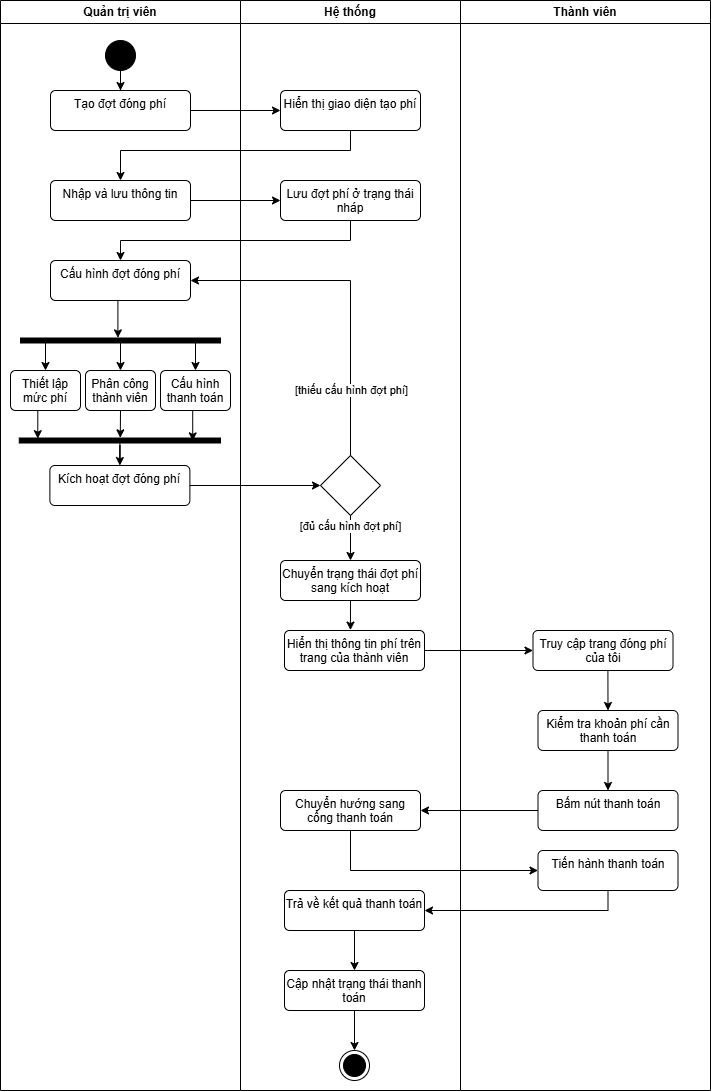
\includegraphics[width=0.75\linewidth]{Images/activity-diagram/payment_acitivity.drawio.png}
        \vspace{0.3em}
        \captionsetup{skip=8pt}
        \caption{Activity Diagram - Quản lý đóng phí}
        \label{fig:activity-uc04}
\end{figure}

Đầu tiên quản trị viên tạo đợt đóng phí theo tổ chức, sau khi bấm lưu đợt đóng phí sẽ được tạo mới ở bản nháp. Để kích hoạt, quản trị viển cần thiết lập mức phí và phân công thành viên. Sau khi đã thiết lập đầy đủ thì hệ thống sẽ cho phép kích hoạt. Khi đợt đóng phí ở trạng thái kích hoạt thì đợt đóng phí sẽ được công bố cho toàn bộ thành viên được phân công có thể xem và thực hiện thanh toán.